\section{Методы повышения эффективности реализации ЭА.}

А нафиг оно надо, если фитнесс считается дольше, чем любые
другие операции ЭА вместе взятые\dots

Однако если посмотреть на мутацию инверсией бита с вероятностью
$1/n$ получаем $n$ вызовов генератора случайных чисел. Кажется
мы зажрались.

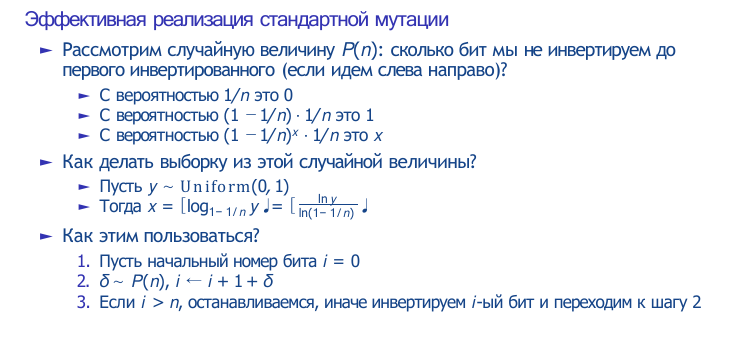
\includegraphics[scale=0.7]{images/38effective_mutation}

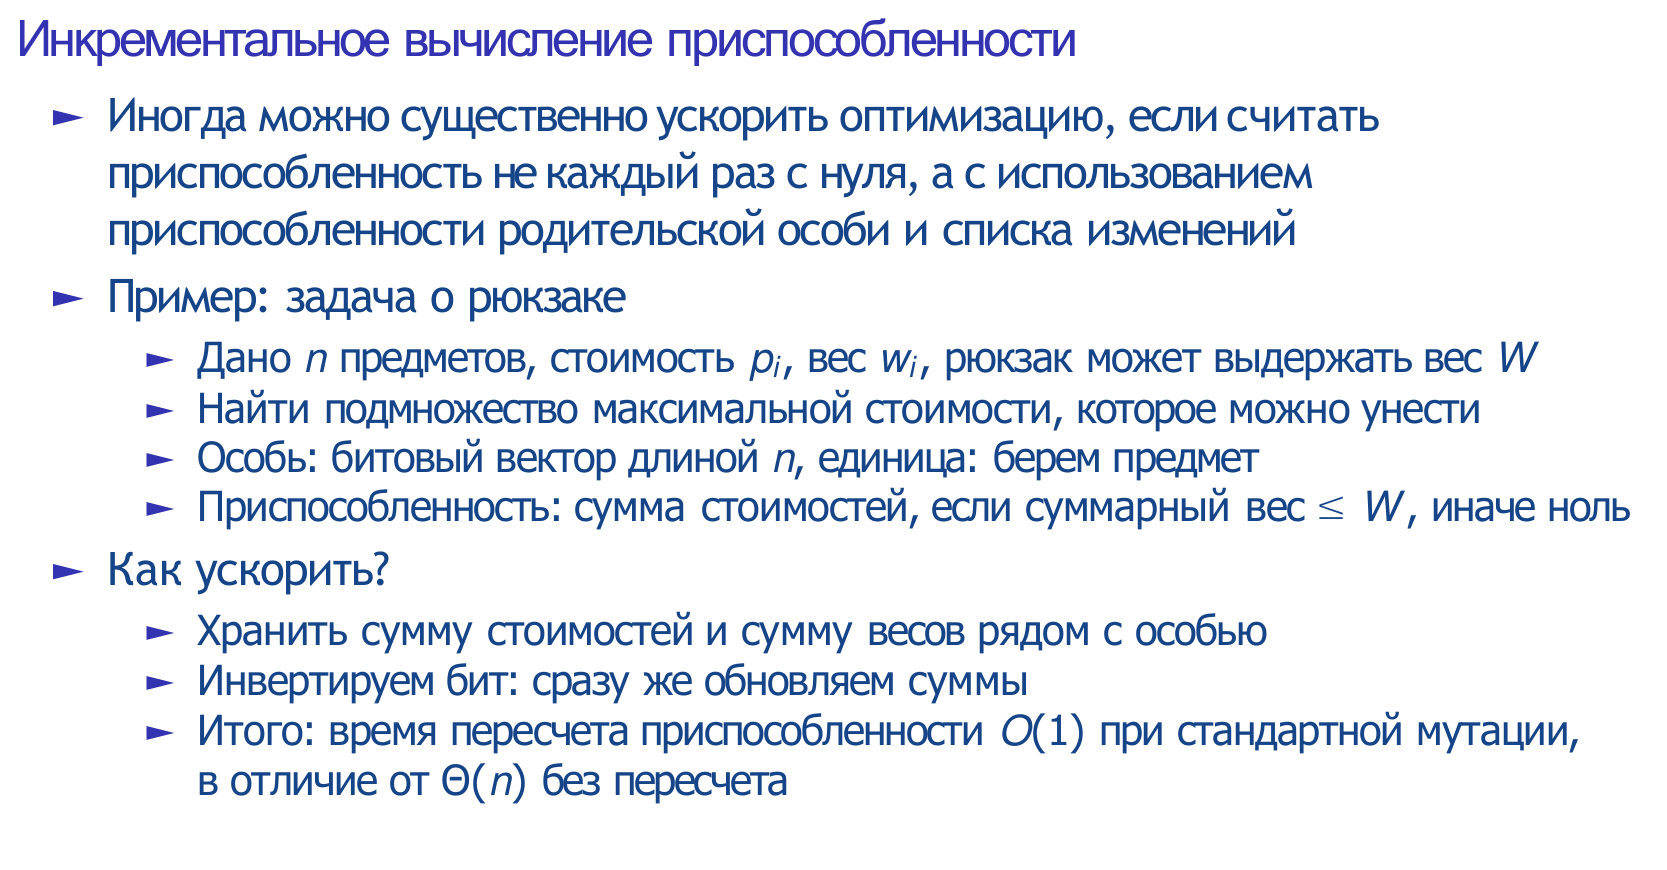
\includegraphics[scale=0.3]{images/38incr_adap}

Продвинутые ЭА используют более сложные алгоритмы внутри.
Особенно это касается многокритериальных алгоритмов. Некоторые
подзадачи являются NP-hard, значит наивные реализации будут
работать слишком долго. Но даже некоторые полиномиальные
подзадачи могут являться узким местом.

Эффективность составных частей определяет эффективность оптимизации
в целом.
